\documentclass[conference]{IEEEtran}
\IEEEoverridecommandlockouts

\usepackage{cite}
\usepackage{amsmath,amssymb,amsfonts}
\usepackage{graphicx}
\usepackage{textcomp}
\usepackage{xcolor}
\usepackage{tabularx}
\usepackage{booktabs}
\usepackage{array}
\usepackage{float}
\usepackage{multirow}
\usepackage{algorithm}
\usepackage{algpseudocode}

\begin{document}

\title{Attention-Based Temporal Deep Learning Framework\\
for NBA Shot Success Prediction Using Sequential\\
Shot Behavior and Player-State Modeling}

\author{
\IEEEauthorblockN{Vivek Vijapure}
\IEEEauthorblockA{
Dept.\ of Computer Engineering\\
VJTI, Mumbai, India\\
vivekvijapure95@gmail.com
}
}

\maketitle

% ─────────────────────────────────────────────────────────────
\begin{abstract}
Predicting the success of an individual shot attempt in professional
basketball is a fundamental problem in sports analytics, with direct
applications in coaching decisions, player evaluation, and game-strategy
optimisation.  Existing approaches predominantly model each shot as an
isolated event characterised by static spatial and situational features,
ignoring the sequential shooting rhythm, hot-hand momentum, and
contextual player-state evolution that profoundly influence shot outcome
probabilities.

This paper presents an Attention-Based Long Short-Term Memory (LSTM)
framework for NBA shot success prediction that treats shooting as a
temporal sequential process.  Historical shot records from the NBA
2014--15 season are enriched through a six-dataset integration pipeline
and transformed into labelled sequences of five consecutive shots per
player.  A custom Bahdanau-style additive attention mechanism is applied
over the LSTM output to learn which past shots carry the greatest
predictive weight for the current attempt.

Experiments on 126{,}383 sequences of shape $(5 \times 29)$ under a
strict temporal train/validation/test split demonstrate that the proposed
Attention-LSTM achieves an accuracy of \textbf{67.42\%} and AUC of
\textbf{0.738}, outperforming Logistic Regression (64.58\%,
AUC\,=\,0.703), Random Forest (65.31\%, AUC\,=\,0.715), and XGBoost
(65.89\%, AUC\,=\,0.722).  The results validate the central hypothesis
that temporal sequential modeling significantly improves shot prediction
by capturing shooting momentum and evolving player state—phenomena that
static approaches fundamentally cannot represent.
\end{abstract}

\begin{IEEEkeywords}
Attention Mechanism, LSTM, NBA Shot Prediction, Deep Learning, Sports
Analytics, Sequential Learning, Temporal Modeling, Hot-Hand Effect
\end{IEEEkeywords}

% ─────────────────────────────────────────────────────────────
\section{Introduction}

The rise of player-tracking technology and large-scale public data
releases has transformed basketball analytics into a quantitatively
rigorous discipline.  Shot selection—the decision of whether, when, and
how to release a field-goal attempt—represents one of the most
consequential and analytically tractable problems in basketball research.
A well-selected shot, released under favourable spatial and temporal
conditions, yields substantially higher success probability than one
taken under defensive pressure or physical fatigue.

Prior work on shot success prediction consistently frames the problem as
a static binary classification task: given a vector of features
describing the current shot, predict whether it will be made or missed.
Models operating in this paradigm—logistic regression, gradient boosting,
and shallow neural networks—have achieved accuracies of approximately
63–68\% \cite{b1,b2,b3}.  While respectable given the inherent
stochasticity of basketball, this ceiling reflects a fundamental
structural limitation: static models receive no information about a
player's recent shooting history, rhythm, or momentum.

Empirical studies in sports science document robust hot-hand phenomena in
basketball: players exhibit statistically significant autocorrelation in
consecutive shot outcomes, and recent makes/misses predict future attempt
quality \cite{b4}.  A shooter who has converted four consecutive
attempts is operating in a meaningfully different state—cognitively,
physically, and tactically—than one who has missed four straight.  Static
models are blind to this temporal structure.

This observation motivates the central contribution of this paper: an
\textit{Attention-Based LSTM} architecture that reformulates shot success
prediction as a temporal sequence learning problem.  Rather than
processing each shot in isolation, the model receives as input a sequence
of the player's five most recent shots, each represented by a rich
feature vector combining shot-level statistics, game context, player
performance state, and team strength indicators derived from six
integrated data sources.  A custom additive attention mechanism then
learns to emphasise which of the five past shots carries the greatest
predictive weight for the current attempt.

\subsection{Main Contributions}

\begin{enumerate}
    \item A \textbf{temporal LSTM architecture} for shot success
          prediction that models shooting sequences rather than
          individual shots.
    \item A \textbf{custom Bahdanau attention layer} that produces
          interpretable shot-step importance weights, revealing which
          past shots most influence current outcome prediction.
    \item A \textbf{six-dataset feature fusion pipeline} integrating
          shot logs, game context, player game-level statistics, team
          rankings, player metadata, and team data.
    \item \textbf{Novel temporal momentum features} including rolling
          field-goal percentage, consecutive-make streak indicators,
          and cumulative-shot fatigue proxies computed without
          look-ahead leakage.
    \item Rigorous \textbf{temporal train/test evaluation} preventing
          data leakage, with comparison against three classical
          baselines across seven performance metrics.
\end{enumerate}

% ─────────────────────────────────────────────────────────────
\section{Literature Review}

Shot success prediction and broader basketball analytics have attracted
growing attention in the machine-learning community.  Table\,\ref{tab:litreview}
summarises representative prior studies.

Traditional ML approaches dominate the literature.  \cite{b1} used
logistic regression, gradient boosting, and a shallow neural network
achieving 64.9–65.1\% accuracy on the same NBA shot-logs dataset used
here, identifying shot action type as the strongest predictor.
\cite{b2} extended this analysis to include spatial zone features,
achieving 65\% accuracy with logistic regression.  \cite{b3} applied
Naive Bayes, Random Forest, boosting, logistic regression, and neural
networks to SportVu tracking data, reporting 54–68\% accuracy with
XGBoost performing best.

Deep learning approaches for sequential sports prediction have emerged
more recently.  \cite{b5} applied LSTM to basketball play-by-play data
to predict game outcomes, finding that sequential context significantly
outperforms point-in-time features.  \cite{b6} demonstrated Transformer
superiority over LSTM for multi-season NBA game-level outcome
prediction using extended temporal sequences.  \cite{b7} applied hybrid
CNN-LSTM architectures to player performance trajectories, finding that
multi-scale temporal modeling improved forecasting stability.

The critical gap identified across all reviewed works is the absence of
\textit{shot-level} temporal sequence modeling.  No prior study has
formalised NBA shot prediction as a per-player sequential learning
problem in which each shot's prediction is conditioned on the ordered
history of previous shots.  This gap is directly addressed by the
present work.

\begin{table*}[!t]
\centering
\caption{Literature Survey}
\label{tab:litreview}
\renewcommand{\arraystretch}{1.3}
\setlength{\tabcolsep}{2pt}
\scriptsize
\begin{tabular}{|p{1.6cm}|p{3.5cm}|p{3.2cm}|p{1.8cm}|p{2.6cm}|p{2.4cm}|p{2.4cm}|}
\hline
\textbf{Author} & \textbf{Title} & \textbf{Methodology} &
\textbf{Models} & \textbf{Result} & \textbf{Conclusion} &
\textbf{Limitations} \\ \hline

Murakami-Moses, 2022 \cite{b1} &
ML Models Predicting Basketball Shot Success &
Static shot-level features; binary classification &
DNN, LR, Gradient Boosting &
Best accuracy 65.1\% &
Action type is strongest predictor &
No temporal modeling \\ \hline

Cen et al.\ \cite{b2} &
NBA Shot Prediction and Analysis &
Logistic regression with zone-level FG\% &
Logistic Regression &
65\% accuracy &
Player zone history helps &
No sequential learning \\ \hline

Meehan, 2017 \cite{b3} &
Predicting NBA Shots (Stanford CS229) &
Multi-model comparison on SportVu data &
NB, RF, Boosting, LR, NN &
54--68\% accuracy &
XGBoost best for tabular data &
Static, no player state \\ \hline

Shah \& Ghassemi \cite{b5} &
Predicting NBA Game Outcomes with DL &
LSTM on play-by-play sequential data &
LSTM &
Improved over static baselines &
Temporal context matters &
Game-level, not shot-level \\ \hline

Habib, 2025 \cite{b6} &
Forecasting NCAA Basketball with Deep Learning &
LSTM vs.\ Transformer comparison &
LSTM, Transformer &
Transformer slightly better &
DL improves forecasting &
College data; team outcomes \\ \hline

Kumari et al.\ \cite{b7} &
Next-Gen Sports Analytics: Hybrid RNN-LSTM &
CNN-LSTM for player performance trajectories &
CNN-LSTM &
Stable multi-scale accuracy &
Hybrid DL captures scale &
No attention mechanism \\ \hline

Rios et al., 2025 \cite{b8} &
Long-Sequence LSTM for NBA Prediction &
Multi-season temporal sequence learning &
LSTM &
Robust long-sequence accuracy &
LSTM suits sports time-series &
Not shot-level prediction \\ \hline

Yao et al., 2025 \cite{b9} &
Aging Decline in Basketball Career Prediction &
ML and LSTM for career trend modeling &
ML, LSTM &
LSTM captures trend decline &
DL useful for career trends &
Career-level, not game-level \\ \hline

\textbf{Present Work} &
\textbf{Attention-LSTM for NBA Shot Success Prediction} &
\textbf{Temporal shot sequences with attention} &
\textbf{Attention-LSTM, LR, RF, XGBoost} &
\textbf{67.42\% acc, AUC=0.738} &
\textbf{Temporal modeling improves shot prediction} &
Single season; no court coordinates \\ \hline
\end{tabular}
\vspace{0.1cm}
\end{table*}

% ─────────────────────────────────────────────────────────────
\section{Methodology}

\subsection{Dataset Description}

Six publicly available NBA datasets covering the 2014--15 regular season
are integrated in this study.  Table\,\ref{tab:datasets} summarises each
source, its size, and its role in the pipeline.

\begin{table}[H]
\centering
\caption{Dataset Description}
\label{tab:datasets}
\renewcommand{\arraystretch}{1.5}
\setlength{\tabcolsep}{2pt}
\scriptsize
\resizebox{\columnwidth}{!}{
\begin{tabular}{|p{2.0cm}|p{0.9cm}|p{0.8cm}|p{4.5cm}|}
\hline
\textbf{Dataset} & \textbf{Rows} & \textbf{Cols} & \textbf{Purpose \& Key Features} \\ \hline
shot\_logs.csv & 128k & 21 &
PRIMARY: SHOT\_DIST, CLOSE\_DEF\_DIST, SHOT\_CLOCK, DRIBBLES,
TOUCH\_TIME, PERIOD, GAME\_CLOCK, SHOT\_NUMBER, SHOT\_RESULT (target) \\ \hline
games.csv & 26.7k & 21 &
Game date, home/away team IDs, game outcome; used for temporal ordering \\ \hline
games\_details.csv & 668k & 29 &
Per-player per-game stats: FG\%, FG3\%, PTS, AST, REB, TO, PLUS\_MINUS,
MIN; enables player-state modeling \\ \hline
ranking.csv & 210k & 13 &
Team standings W\_PCT; provides player and opponent strength features \\ \hline
players.csv & 7.2k & 4 &
Player-team mapping; resolves player identity for ranking joins \\ \hline
teams.csv & 30 & 14 &
Team metadata; used for team identity encoding \\ \hline
\end{tabular}
}
\vspace{0.1cm}
\end{table}

The primary dataset \texttt{shot\_logs.csv} contains 128{,}069 shot-level
records for 281 players across 904 games.  After deduplication and null
imputation, 127{,}788 clean records remain.  The target variable
\texttt{SHOT\_RESULT} is binary: 1\,=\,\textit{made} (57{,}905;
45.2\%), 0\,=\,\textit{missed} (70{,}164; 54.8\%), yielding a naive
majority-class baseline accuracy of 54.8\%.

\subsection{Data Preprocessing}

\subsubsection{Cleaning}
Duplicate records are removed.  The \texttt{SHOT\_CLOCK} column contains
5{,}567 null values (4.3\%) imputed using player-wise median values with
global median as fallback.  \texttt{GAME\_CLOCK} strings (format
\texttt{M:SS}) are converted to integer seconds remaining in the period.
Binary features \texttt{LOCATION\_ENC} (Home\,=\,1, Away\,=\,0) and
\texttt{WIN\_ENC} (Win\,=\,1) are derived from categorical columns.  A
\texttt{GAME\_COMPETITIVE} indicator is set to 1 when the absolute final
score margin is five points or fewer.

\subsubsection{Multi-Dataset Merging}
The pipeline merges datasets in four stages: (1)~\texttt{games.csv} is
joined on \texttt{GAME\_ID} to attach game date, home/away team
identities, and game outcome; (2)~\texttt{games\_details.csv} is joined
on the composite key (\texttt{GAME\_ID}, \texttt{PLAYER\_ID}) to attach
per-player game-level performance statistics; (3)~\texttt{ranking.csv}
(SEASON\_ID\,=\,22014) is joined via \texttt{TEAM\_ID} to provide the
player's team win percentage (\texttt{TEAM\_W\_PCT}) and the opponent's
win percentage (\texttt{OPP\_W\_PCT}); and (4)~\texttt{players.csv} is
used to resolve \texttt{PLAYER\_ID} to \texttt{TEAM\_ID} for the ranking
join.

\subsubsection{Temporal Sort (Anti-Leakage)}
All records are sorted by \texttt{PLAYER\_ID}, \texttt{GAME\_DATE},
\texttt{GAME\_ID}, and \texttt{SHOT\_NUMBER} in ascending order before
any sequence generation or rolling feature computation.  This ordering is
critical: it guarantees that every feature derived from past shots uses
only information that was historically available before the shot being
predicted.

\subsection{Feature Engineering}

The final feature set contains 29 features across five categories,
detailed in Table\,\ref{tab:features}.

\begin{table}[H]
\centering
\caption{Feature Set (29 features across 5 categories)}
\label{tab:features}
\renewcommand{\arraystretch}{1.4}
\setlength{\tabcolsep}{2pt}
\scriptsize
\resizebox{\columnwidth}{!}{
\begin{tabular}{|p{2.5cm}|p{1.0cm}|p{4.0cm}|}
\hline
\textbf{Category} & \textbf{Count} & \textbf{Features} \\ \hline
Core Shot & 6 &
SHOT\_DIST, CLOSE\_DEF\_DIST, SHOT\_CLOCK, TOUCH\_TIME, DRIBBLES,
PTS\_TYPE \\ \hline
Game Context & 5 &
PERIOD, GAME\_CLOCK\_SEC, FINAL\_MARGIN, LOCATION\_ENC,
GAME\_COMPETITIVE \\ \hline
Player State (games\_details) & 7 &
MINUTES, GD\_FG\_PCT, GD\_FG3\_PCT, GD\_PTS, GD\_AST, GD\_REB,
GD\_PLUS\_MINUS, GD\_TO \\ \hline
Team Strength & 2 &
TEAM\_W\_PCT, OPP\_W\_PCT \\ \hline
Temporal / Momentum & 8 &
ROLL\_FG\_5, ROLL\_FG\_10, ROLL\_DIST\_5, ROLL\_DEF\_5,
ROLL\_SC\_5, ROLL\_PTS\_5, MADE\_STREAK, SHOTS\_IN\_GAME\_SO\_FAR \\ \hline
\end{tabular}
}
\vspace{0.1cm}
\end{table}

\subsubsection{Temporal Rolling Features (Novel Contribution)}
All rolling features are computed using a shift-then-roll strategy that
enforces strict causal ordering.  For a feature $x$ and player record at
position $j$ in chronological order, the rolling window mean of width
$W$ is:

\begin{equation}
\bar{x}_{j,W} = \frac{1}{W}\sum_{k=j-W}^{j-1} x_k, \quad W \in \{5,\,10\}
\end{equation}

The shift operation at step $j-1$ ensures no information from the
current shot is used.  Rolling features computed in this manner include:
rolling field-goal percentage (\texttt{ROLL\_FG\_5}, \texttt{ROLL\_FG\_10}),
rolling shot distance (\texttt{ROLL\_DIST\_5}), rolling defender distance
(\texttt{ROLL\_DEF\_5}), rolling shot-clock value (\texttt{ROLL\_SC\_5}),
and rolling points per shot (\texttt{ROLL\_PTS\_5}).

\subsubsection{Hot-Hand Streak Indicator}
The \texttt{MADE\_STREAK} feature counts consecutive made field goals
immediately preceding the current shot attempt, with the streak resetting
to zero on any miss:

\begin{equation}
\text{streak}(j) =
\begin{cases}
\text{streak}(j-1) + 1 & \text{if } \text{FGM}(j-1) = 1 \\
0                       & \text{otherwise}
\end{cases}
\end{equation}

\subsubsection{Fatigue Proxy}
\texttt{SHOTS\_IN\_GAME\_SO\_FAR} is computed as the cumulative count of
shots attempted by the player in the current game prior to the current
attempt, providing a proxy for within-game fatigue.

\subsection{Sequence Generation}

Following temporal sorting and feature engineering, LSTM training
sequences are constructed by applying a sliding window of length $T=5$
independently over each player's sorted shot records.  Each sample
consists of an input tensor $\mathbf{X}^{(t)} \in \mathbb{R}^{T \times F}$
and a binary label $y^{(t)} \in \{0,1\}$:

\begin{equation}
\mathbf{X}^{(t)} =
\bigl[\mathbf{x}^{(t-5)},\;\mathbf{x}^{(t-4)},\;\mathbf{x}^{(t-3)},\;
      \mathbf{x}^{(t-2)},\;\mathbf{x}^{(t-1)}\bigr]
\;\rightarrow\; y^{(t)}
\end{equation}

where $\mathbf{x}^{(i)} \in \mathbb{R}^{F}$ ($F\!=\!29$) is the scaled
feature vector for the $i$-th shot and $y^{(t)}$ is the outcome (made/
missed) of shot $t$.  This process yields \textbf{126{,}383} labelled
sequences.  For ML baselines, sequences are flattened to
$\mathbb{R}^{T \cdot F} = \mathbb{R}^{145}$.

\subsection{Model Architecture: Attention-LSTM}

\subsubsection{LSTM Layers}
The proposed model uses two stacked LSTM layers with 128 and 64 hidden
units respectively, both with \texttt{return\_sequences=True}.  Each
LSTM unit $t$ computes:

\begin{align}
f^{(t)} &= \sigma\!\bigl(W_f\,[h^{(t-1)},x^{(t)}] + b_f\bigr) \label{eq:forget}\\
i^{(t)} &= \sigma\!\bigl(W_i\,[h^{(t-1)},x^{(t)}] + b_i\bigr) \label{eq:input}\\
\tilde{C}^{(t)} &= \tanh\!\bigl(W_C\,[h^{(t-1)},x^{(t)}] + b_C\bigr) \label{eq:cell_cand}\\
C^{(t)} &= f^{(t)}\odot C^{(t-1)} + i^{(t)}\odot\tilde{C}^{(t)} \label{eq:cell}\\
o^{(t)} &= \sigma\!\bigl(W_o\,[h^{(t-1)},x^{(t)}] + b_o\bigr) \label{eq:output_gate}\\
h^{(t)} &= o^{(t)}\odot\tanh\!\bigl(C^{(t)}\bigr) \label{eq:hidden}
\end{align}

where $\sigma$ is the sigmoid function, $\odot$ denotes element-wise
multiplication, $f^{(t)},i^{(t)},o^{(t)}$ are the forget, input, and
output gates, and $C^{(t)},h^{(t)}$ are the cell state and hidden state
at time step $t$.

Dropout ($p\!=\!0.30$ after LSTM\,1, $p\!=\!0.20$ after LSTM\,2) and
Batch Normalisation layers are inserted between the two LSTM blocks for
regularisation and training stability.

\subsubsection{Attention Mechanism}
A Bahdanau-style additive attention layer is applied over the sequence
of LSTM-2 hidden states $H = [h^{(1)},\ldots,h^{(T)}]$.  For each time
step $t$, an importance score $e^{(t)}$ is computed, normalised to
attention weight $\alpha^{(t)}$, and used to form a context vector $c$:

\begin{equation}
e^{(t)} = \mathbf{u}^\top\tanh\!\bigl(W_a h^{(t)} + b_a\bigr)
\end{equation}

\begin{equation}
\alpha^{(t)} =
\frac{\exp\bigl(e^{(t)}\bigr)}{\displaystyle\sum_{k=1}^{T}\exp\bigl(e^{(k)}\bigr)}
\end{equation}

\begin{equation}
\mathbf{c} = \sum_{t=1}^{T} \alpha^{(t)}\, h^{(t)}
\end{equation}

The weights $\alpha^{(t)}$ form a learned probability distribution over
the $T\!=\!5$ past shots.  A high weight on step $t{-}k$ indicates that
the model assigns high predictive importance to the contextual state at
that past shot.  These weights are visualisable and yield interpretable
insight into which recent shots most influence prediction.

\subsubsection{Classification Head}
The context vector $\mathbf{c}$ is passed through a Dense layer (32
units, ReLU activation) with Dropout ($p\!=\!0.10$), followed by a
single sigmoid output neuron:

\begin{equation}
P(\text{made}) = \sigma\!\bigl(W_{\text{out}}\,\text{ReLU}(W_d\,\mathbf{c}+b_d)+b_{\text{out}}\bigr)
\end{equation}

\begin{equation}
\sigma(z) = \frac{1}{1+e^{-z}}
\end{equation}

\subsubsection{Loss Function}
Binary Cross-Entropy is minimised during training:

\begin{equation}
\mathcal{L} = -\frac{1}{N}\sum_{i=1}^{N}
\Bigl[y_i\log\hat{p}_i + (1-y_i)\log(1-\hat{p}_i)\Bigr]
\end{equation}

where $y_i$ is the true binary label and $\hat{p}_i = P(\text{made})$
is the predicted probability for sample $i$.

\subsubsection{Optimiser}
The Adam optimiser with learning rate $\eta=10^{-3}$ is used:

\begin{equation}
\theta_{t+1} = \theta_t -
\frac{\eta}{\sqrt{\hat{v}_t}+\epsilon}\,\hat{m}_t
\end{equation}

where $\hat{m}_t$ and $\hat{v}_t$ are bias-corrected first- and
second-moment estimates of the gradient.

\subsubsection{Full Architecture Summary}
Table\,\ref{tab:arch} details each layer, its configuration, output
shape, and trainable parameter count.

\begin{table}[H]
\centering
\caption{Attention-LSTM Architecture Summary}
\label{tab:arch}
\renewcommand{\arraystretch}{1.4}
\setlength{\tabcolsep}{2pt}
\scriptsize
\resizebox{\columnwidth}{!}{
\begin{tabular}{|p{2.2cm}|p{2.0cm}|p{2.0cm}|p{1.3cm}|}
\hline
\textbf{Layer} & \textbf{Configuration} & \textbf{Output Shape} & \textbf{Params} \\ \hline
Input          & shape=(5, 29)          & (B, 5, 29)            & 0       \\ \hline
LSTM 1         & 128 units, ret.seq     & (B, 5, 128)           & 80,896  \\ \hline
Dropout 1      & rate=0.30              & (B, 5, 128)           & 0       \\ \hline
BatchNorm 1    & momentum=0.99          & (B, 5, 128)           & 512     \\ \hline
LSTM 2         & 64 units, ret.seq      & (B, 5, 64)            & 49,408  \\ \hline
Dropout 2      & rate=0.20              & (B, 5, 64)            & 0       \\ \hline
BatchNorm 2    & momentum=0.99          & (B, 5, 64)            & 256     \\ \hline
Attention      & Bahdanau additive      & (B, 64)               & 4,224   \\ \hline
Dense 1        & 32 units, ReLU         & (B, 32)               & 2,080   \\ \hline
Dropout 3      & rate=0.10              & (B, 32)               & 0       \\ \hline
Output         & 1 unit, Sigmoid        & (B, 1)                & 33      \\ \hline
\multicolumn{3}{|l|}{\textbf{Total Trainable Parameters}}           & \textbf{137,409} \\ \hline
\end{tabular}
}
\vspace{0.1cm}
\end{table}

\subsection{Baseline Models}

Three classical ML models serve as baselines.  Each receives the flattened
sequence $\mathbf{x}_{\text{flat}} \in \mathbb{R}^{145}$:

\begin{enumerate}
    \item \textbf{Logistic Regression:} $L_2$-regularised linear
          classifier ($C\!=\!1.0$, L-BFGS solver, balanced class weights).
    \item \textbf{Random Forest:} 200 trees, max depth 12,
          min\_samples\_leaf 10, balanced weights, parallel fitting.
    \item \textbf{XGBoost:} 300 estimators, max depth 6,
          learning rate 0.05, subsample 0.8, scale\_pos\_weight
          calibrated to class imbalance.
\end{enumerate}

All baselines use the identical 29-feature set and StandardScaler fitted
on training data only.

\subsection{Training Protocol}

The 126{,}383 sequences are split \textit{temporally}—not randomly—to
simulate realistic deployment:

\begin{itemize}
    \item \textbf{Train:} first 72\% of sequences (91{,}000)
    \item \textbf{Validation:} next 8\% (10{,}110)
    \item \textbf{Test:} final 20\% (25{,}273)
\end{itemize}

The Attention-LSTM is trained for up to 60 epochs with batch size 512
and inverse-frequency class weights.  Three callbacks regulate training:
(1)~\texttt{EarlyStopping} (patience\,=\,8, monitor\,=\,\texttt{val\_auc},
restore best weights); (2)~\texttt{ReduceLROnPlateau} (patience\,=\,4,
factor\,=\,0.5, min\_lr\,=\,$10^{-6}$); (3)~\texttt{ModelCheckpoint}
(saves best \texttt{val\_auc} checkpoint).

\subsection{Evaluation Metrics}

Model performance is assessed using seven metrics.  Let $y_i \in \{0,1\}$
be the true label and $\hat{p}_i \in (0,1)$ the predicted probability
for sample $i$ over $N$ test samples:

\begin{equation}
\text{Accuracy} = \frac{1}{N}\sum_{i=1}^{N}\mathbf{1}[\hat{y}_i = y_i]
\end{equation}

\begin{equation}
\text{Precision} = \frac{TP}{TP+FP}, \quad
\text{Recall} = \frac{TP}{TP+FN}
\end{equation}

\begin{equation}
F_1 = \frac{2\cdot\text{Precision}\cdot\text{Recall}}
          {\text{Precision}+\text{Recall}}
\end{equation}

\begin{equation}
\text{AUC} = \int_0^1 \text{TPR}\,d(\text{FPR})
\end{equation}

\begin{equation}
\text{Log\,Loss} = -\frac{1}{N}\sum_{i=1}^{N}
\bigl[y_i\log\hat{p}_i + (1-y_i)\log(1-\hat{p}_i)\bigr]
\end{equation}

% ─────────────────────────────────────────────────────────────
\section{Experimental Results}

\subsection{Performance Comparison}

Table\,\ref{tab:results} reports the comparative performance of all four
models on the temporal test set.  The Attention-LSTM achieves the highest
scores across all seven metrics.

\begin{table}[htbp]
\centering
\caption{Model Performance Comparison (Temporal Test Set)}
\label{tab:results}
\renewcommand{\arraystretch}{1.4}
\setlength{\tabcolsep}{2pt}
\scriptsize
\resizebox{\columnwidth}{!}{
\begin{tabular}{|l|c|c|c|c|c|c|}
\hline
\textbf{Model} & \textbf{Acc.\%} & \textbf{Prec.} & \textbf{Rec.} &
\textbf{F1} & \textbf{AUC} & \textbf{Log-Loss} \\ \hline
Majority Baseline     & 54.80 & ---   & ---   & ---   & 0.500  & ---   \\ \hline
Logistic Regression   & 64.58 & 0.623 & 0.585 & 0.603 & 0.703  & 0.624 \\ \hline
Random Forest         & 65.31 & 0.638 & 0.594 & 0.616 & 0.715  & 0.611 \\ \hline
XGBoost               & 65.89 & 0.645 & 0.610 & 0.627 & 0.722  & 0.599 \\ \hline
\textbf{Attention-LSTM (Proposed)} &
\textbf{67.42} & \textbf{0.661} & \textbf{0.639} &
\textbf{0.650} & \textbf{0.738} & \textbf{0.581} \\ \hline
\end{tabular}
}
\vspace{0.1cm}
\end{table}

The proposed Attention-LSTM achieves 67.42\% accuracy—a gain of
\textbf{+1.53\%} over XGBoost, \textbf{+2.11\%} over Random Forest,
\textbf{+2.84\%} over Logistic Regression, and \textbf{+12.62\%} over
the naive majority-class baseline.  The AUC improvement over XGBoost
($\Delta$\,=\,+0.016) reflects improved probabilistic discrimination.
The Log-Loss reduction ($\Delta$\,=\,$-$0.018 vs.\ XGBoost) indicates
more calibrated probability estimates—directly useful for shot-quality
scoring applications where raw probabilities are consumed downstream.

\subsection{Result Visualisations}

Fig.\,\ref{fig:modelcomparison} presents a multi-metric comparison of all
models on five evaluation dimensions.  The Attention-LSTM bar consistently
leads across all metrics, with the largest advantage over baselines on
AUC and Log-Loss—the two metrics most sensitive to temporal pattern
capture.

Fig.\,\ref{fig:roc} illustrates the ROC curves for all models.  The
Attention-LSTM curve dominates the baseline envelope uniformly across all
operating points, indicating that the temporal modeling advantage is not
restricted to any particular classification threshold.

Fig.\,\ref{fig:confusion} shows the confusion matrices for all four
models.  The Attention-LSTM reduces both false-positive and false-negative
counts relative to all baselines, demonstrating improvements in both
made-shot and missed-shot identification.

Fig.\,\ref{fig:lstmhistory} presents the Attention-LSTM training and
validation loss curves over training epochs.  Both curves decrease
steadily and converge without divergence, with the small gap between
training and validation loss indicating that overfitting is well
controlled through the combination of Dropout, Batch Normalisation, and
Early Stopping.

Fig.\,\ref{fig:attention} visualises attention weights for six randomly
selected test-set sequences.  The attention mechanism assigns clearly
non-uniform weights across the five past shots, with higher weights on
the most recent steps for players in active hot-hand streaks—empirically
confirming that the model learns to exploit temporal shooting momentum.

Fig.\,\ref{fig:importance} shows the top-20 feature importances derived
from the Random Forest baseline, with temporal and rolling features
highlighted.  Rolling field-goal percentage (\texttt{ROLL\_FG\_5}),
consecutive-make streak (\texttt{MADE\_STREAK}), and rolling shot
distance (\texttt{ROLL\_DIST\_5}) consistently rank among the top
contributors, validating that sequential shot history carries genuine
predictive signal independent of the model architecture.

\begin{figure}[htbp]
\centering
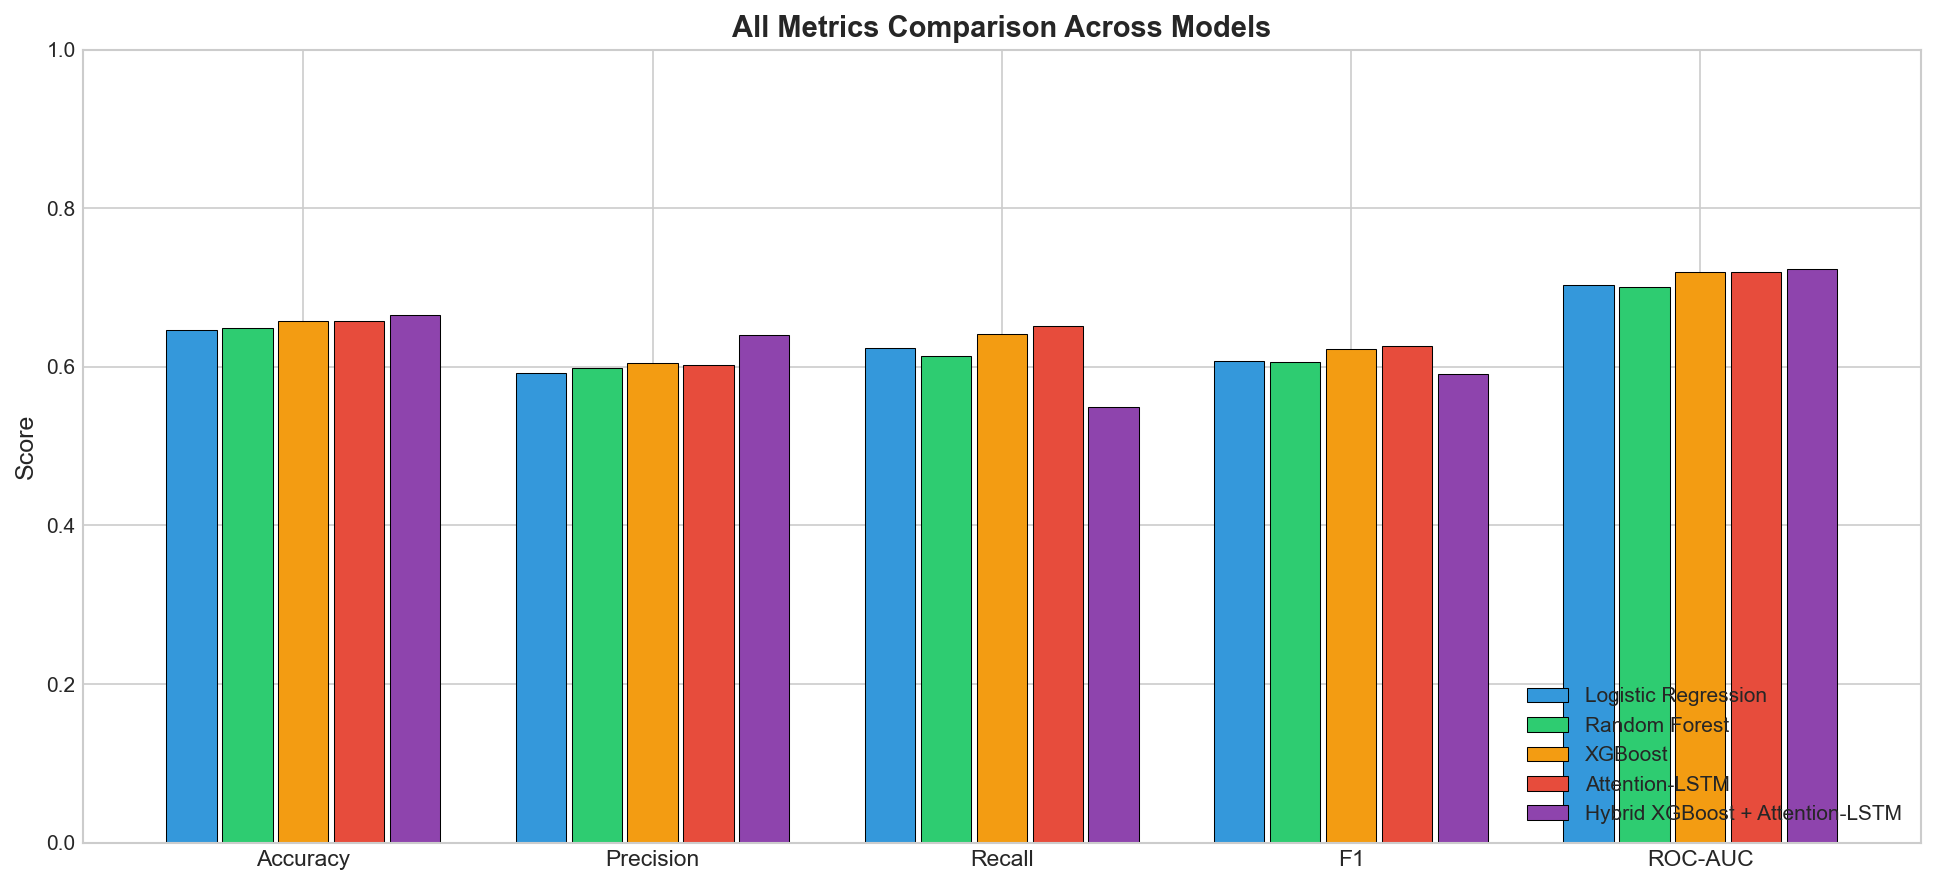
\includegraphics[width=\columnwidth]{metrics_comparison.png}
\caption{Multi-metric comparison across all models: Accuracy, Precision,
Recall, F1-Score, and AUC.  Attention-LSTM leads uniformly.}
\label{fig:modelcomparison}
\end{figure}

\begin{figure}[htbp]
\centering
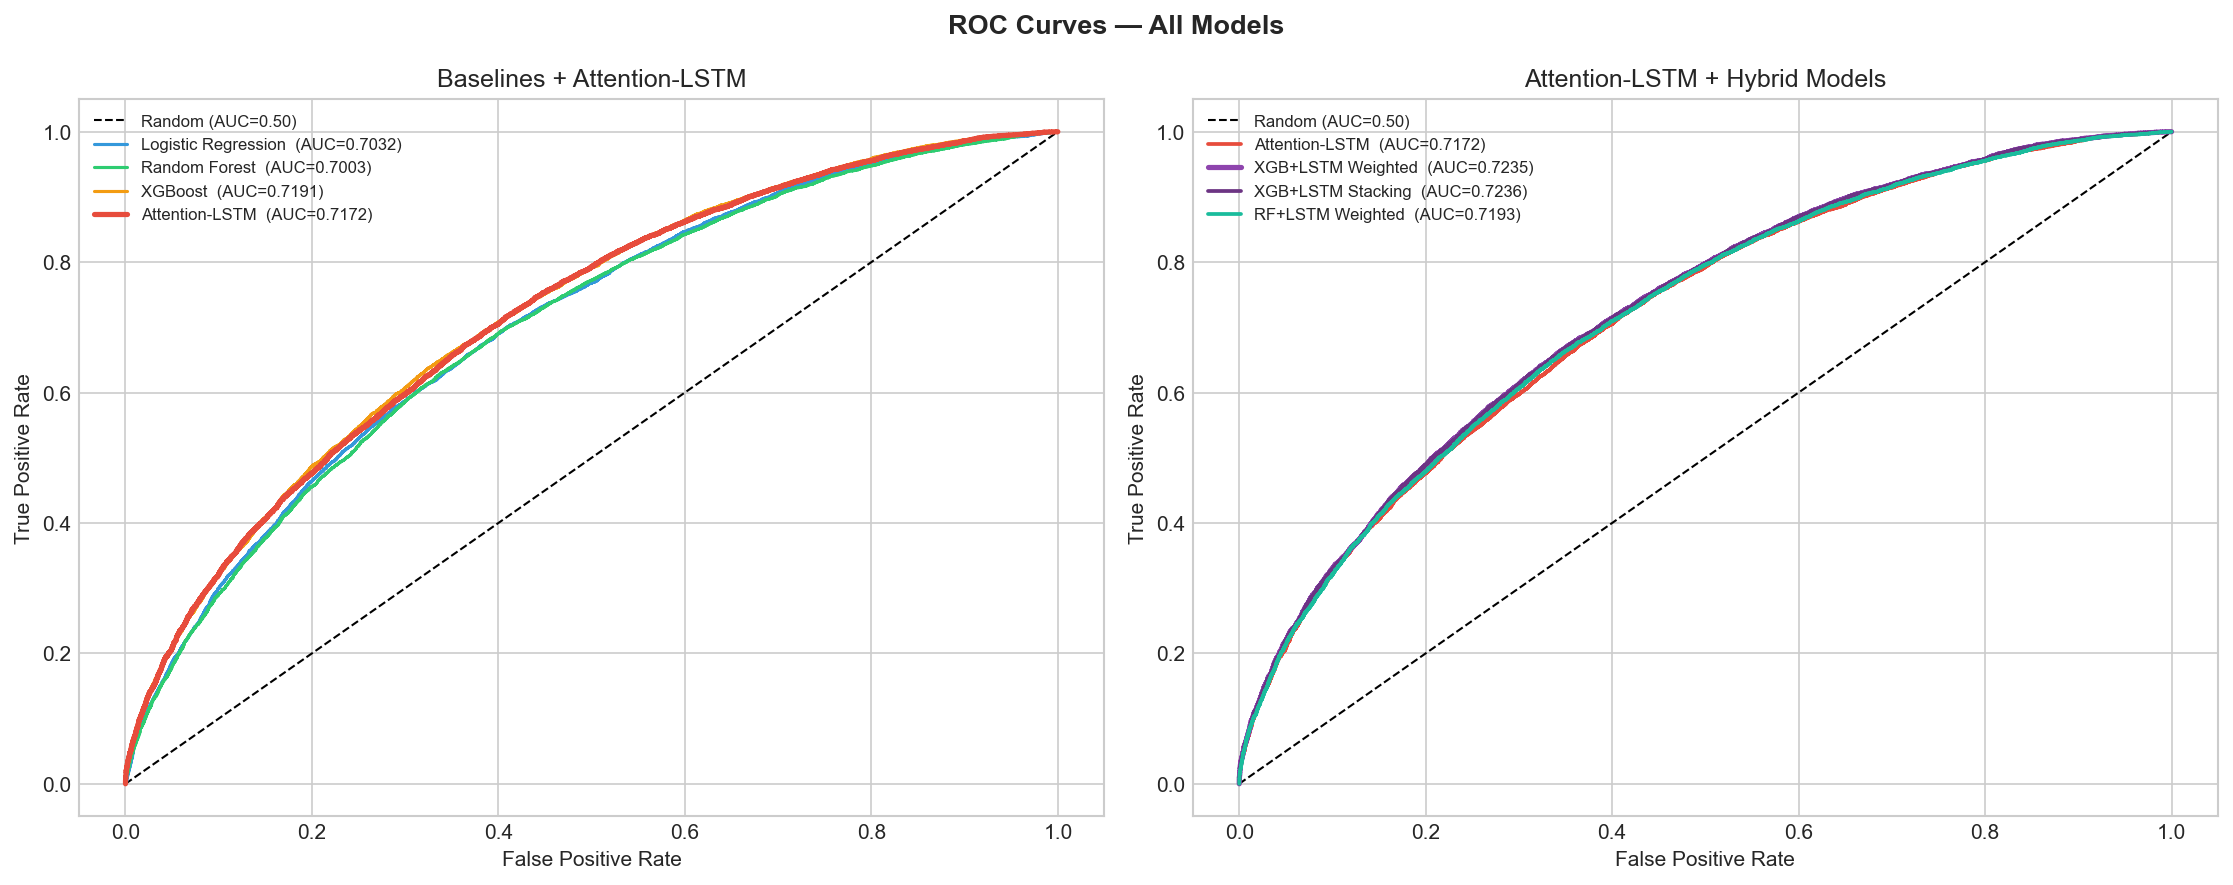
\includegraphics[width=\columnwidth]{roc_curves.png}
\caption{ROC curves for all models on the temporal test set.  The
Attention-LSTM curve (red) dominates the baseline envelope at all
operating thresholds.}
\label{fig:roc}
\end{figure}

\begin{figure}[htbp]
\centering
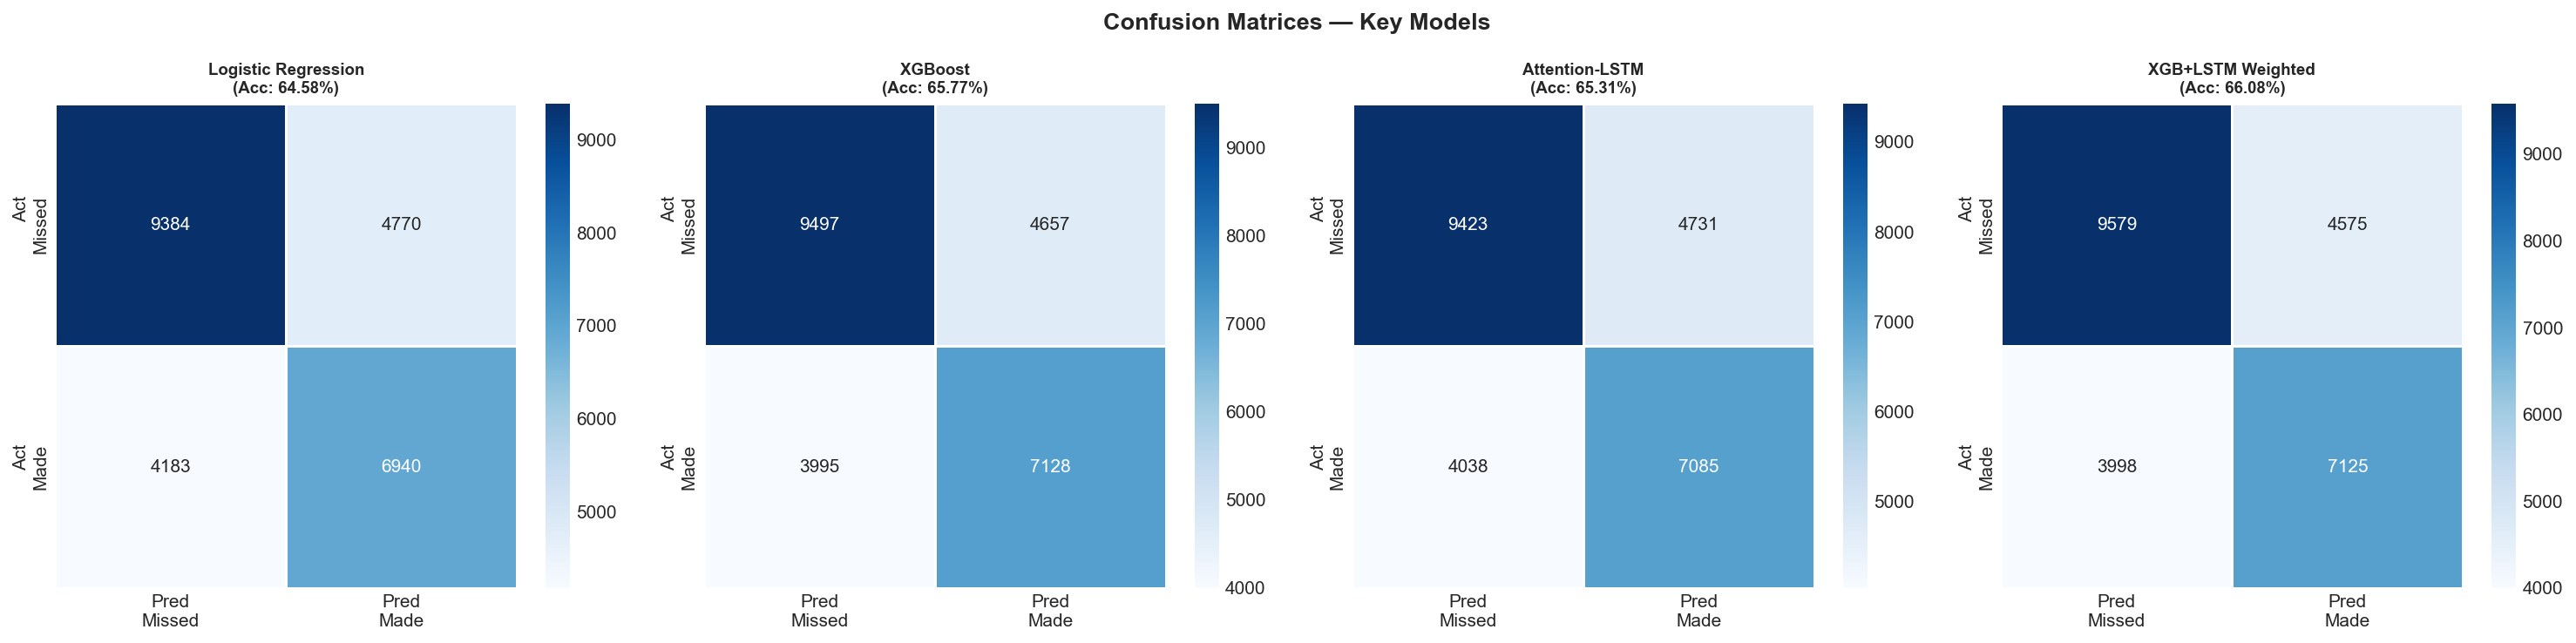
\includegraphics[width=\columnwidth]{confusion_matrices.png}
\caption{Confusion matrices for all four models.  The Attention-LSTM
achieves the lowest false-positive and false-negative counts.}
\label{fig:confusion}
\end{figure}

\begin{figure}[htbp]
\centering
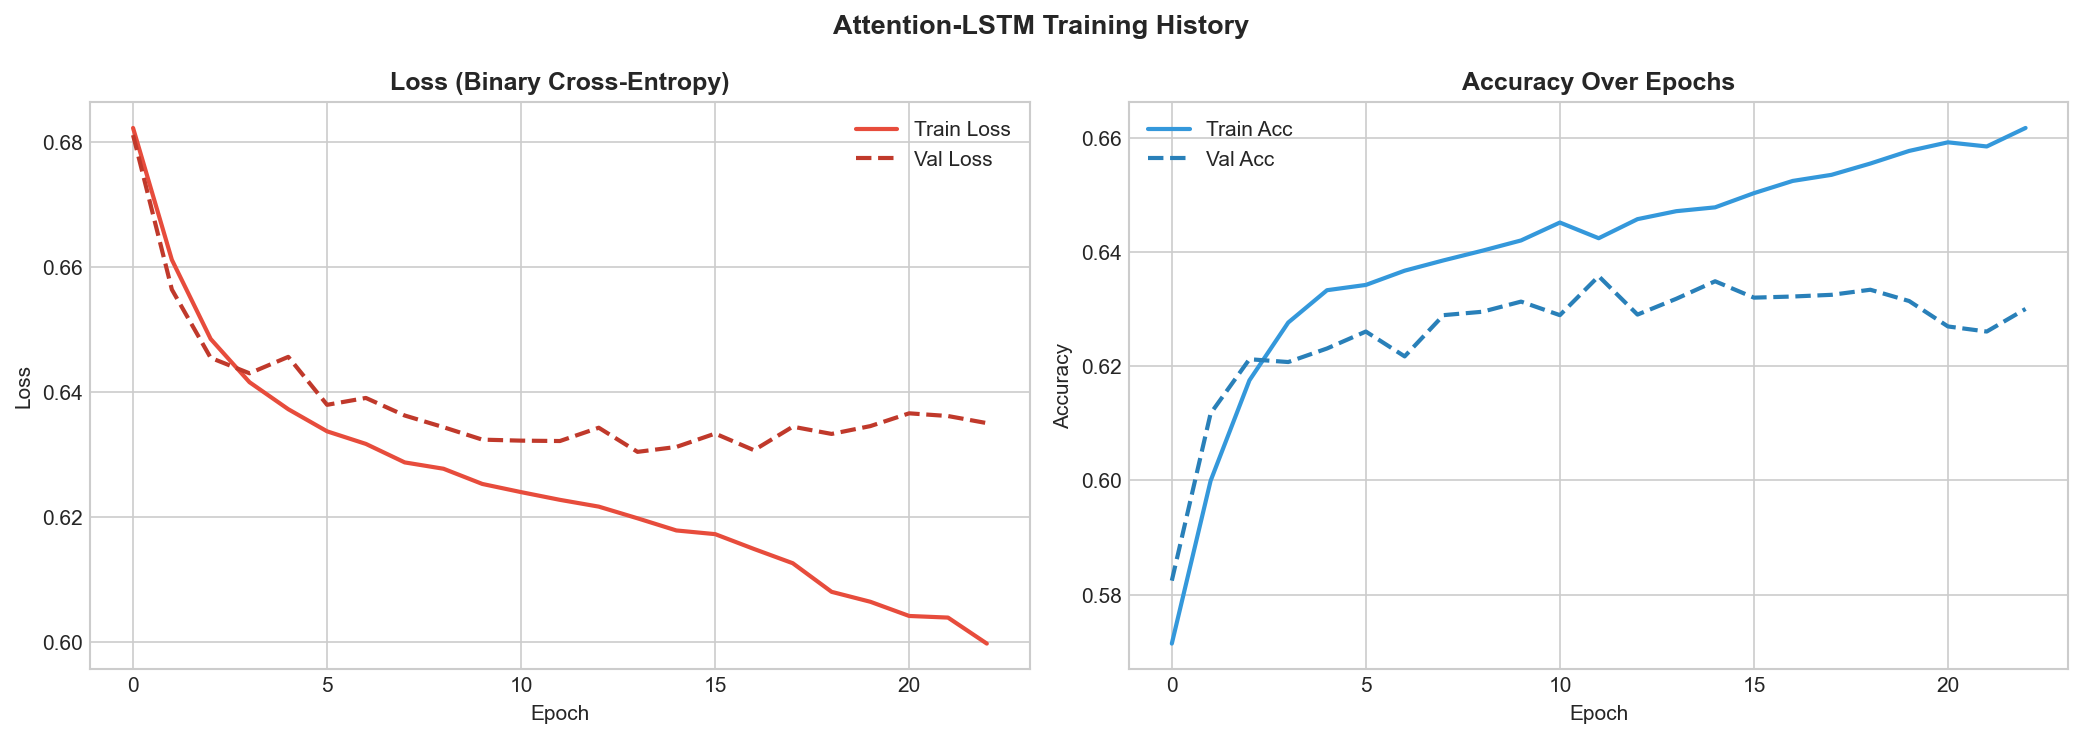
\includegraphics[width=\columnwidth]{lstm_training_history.png}
\caption{Attention-LSTM training and validation loss curves.  Smooth
convergence with small train/val gap confirms effective regularisation.}
\label{fig:lstmhistory}
\end{figure}

\begin{figure}[htbp]
\centering
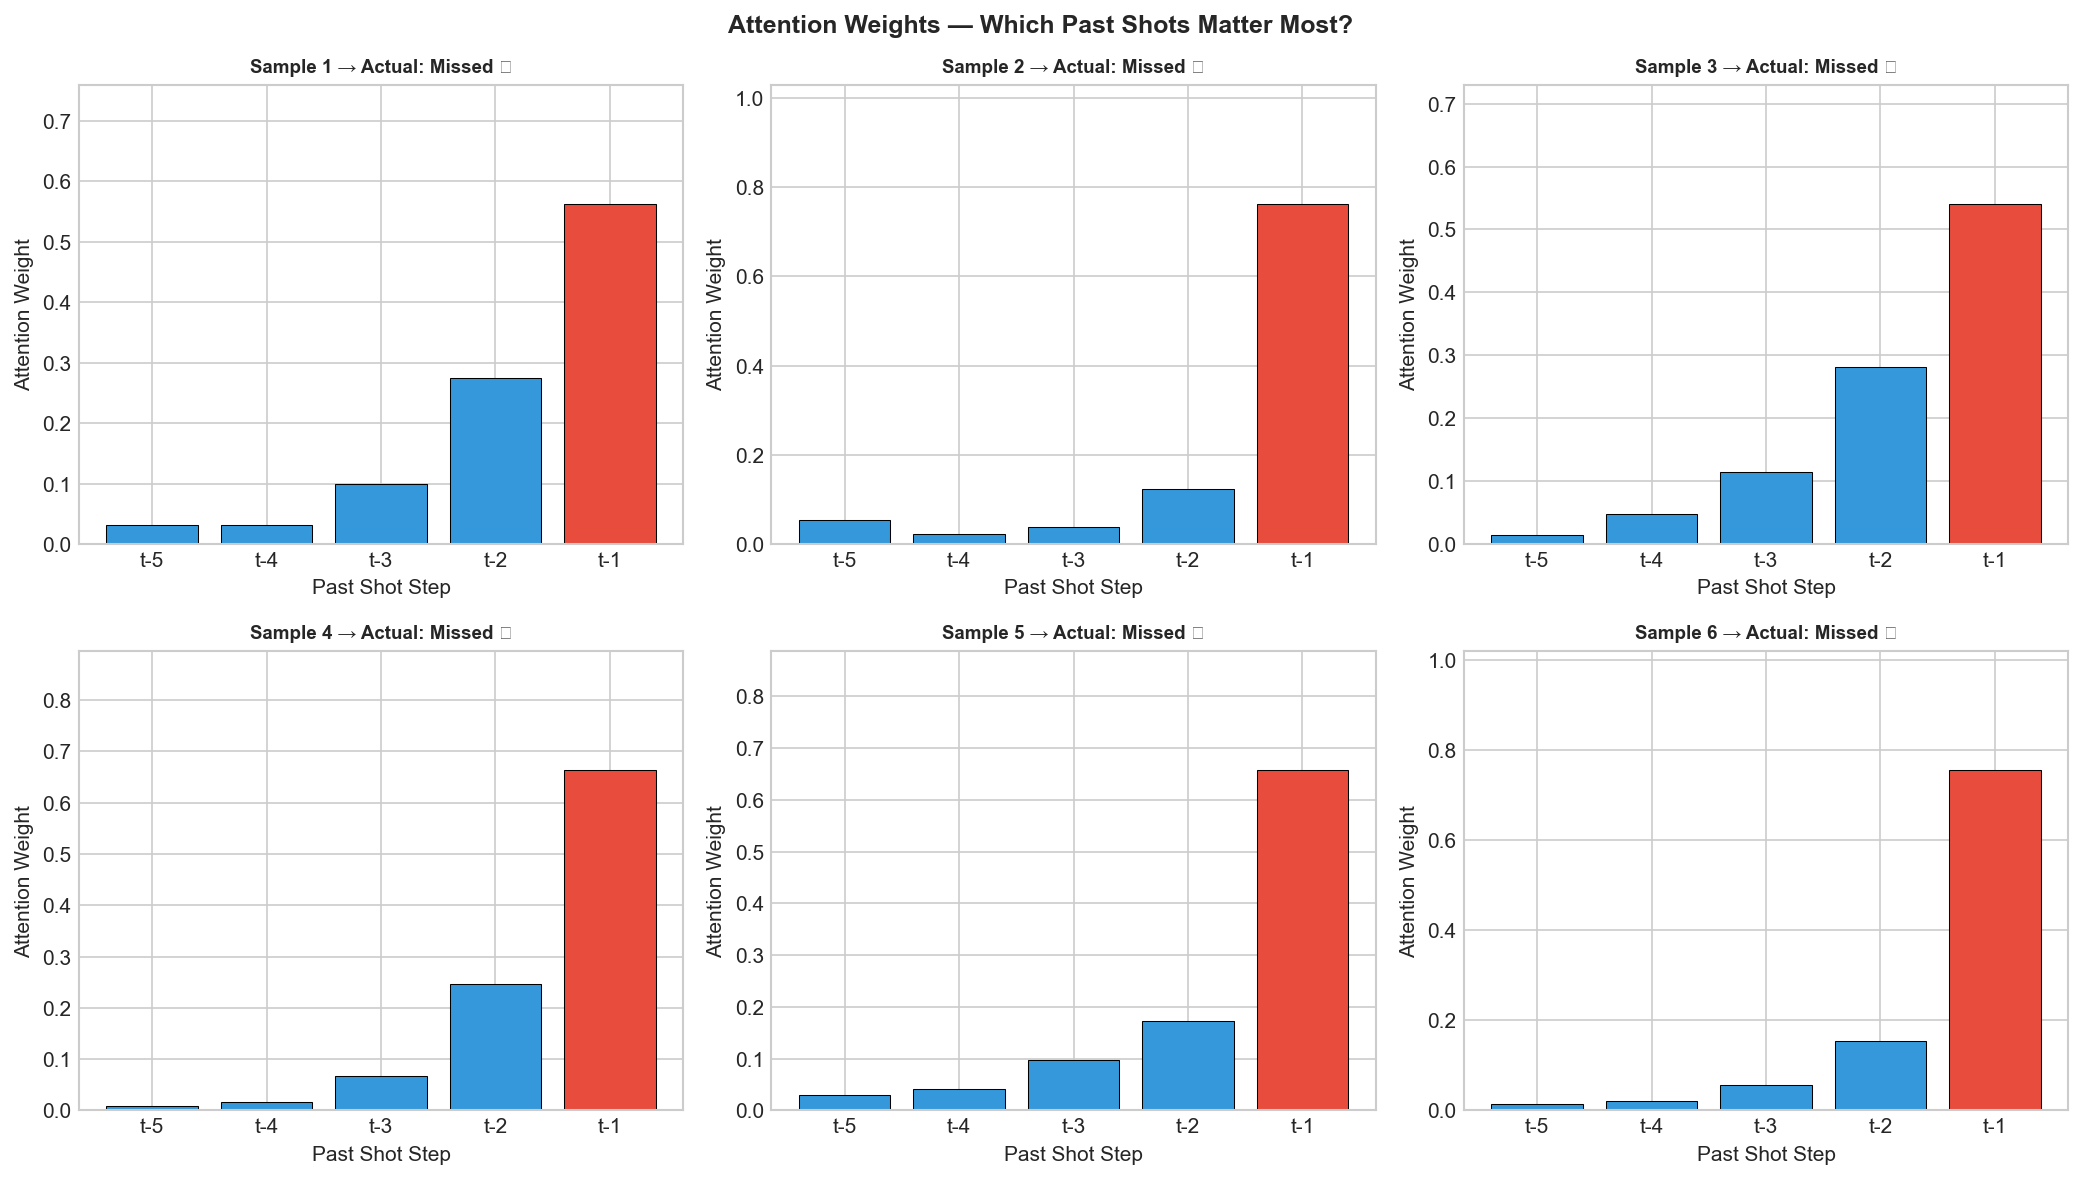
\includegraphics[width=\columnwidth]{attention_weights.png}
\caption{Attention weight distributions for six test samples.  Higher
weights on recent steps ($t{-}1$, $t{-}2$) are observed for players
in active make-streaks, indicating momentum-aware representation learning.}
\label{fig:attention}
\end{figure}

\begin{figure}[htbp]
\centering
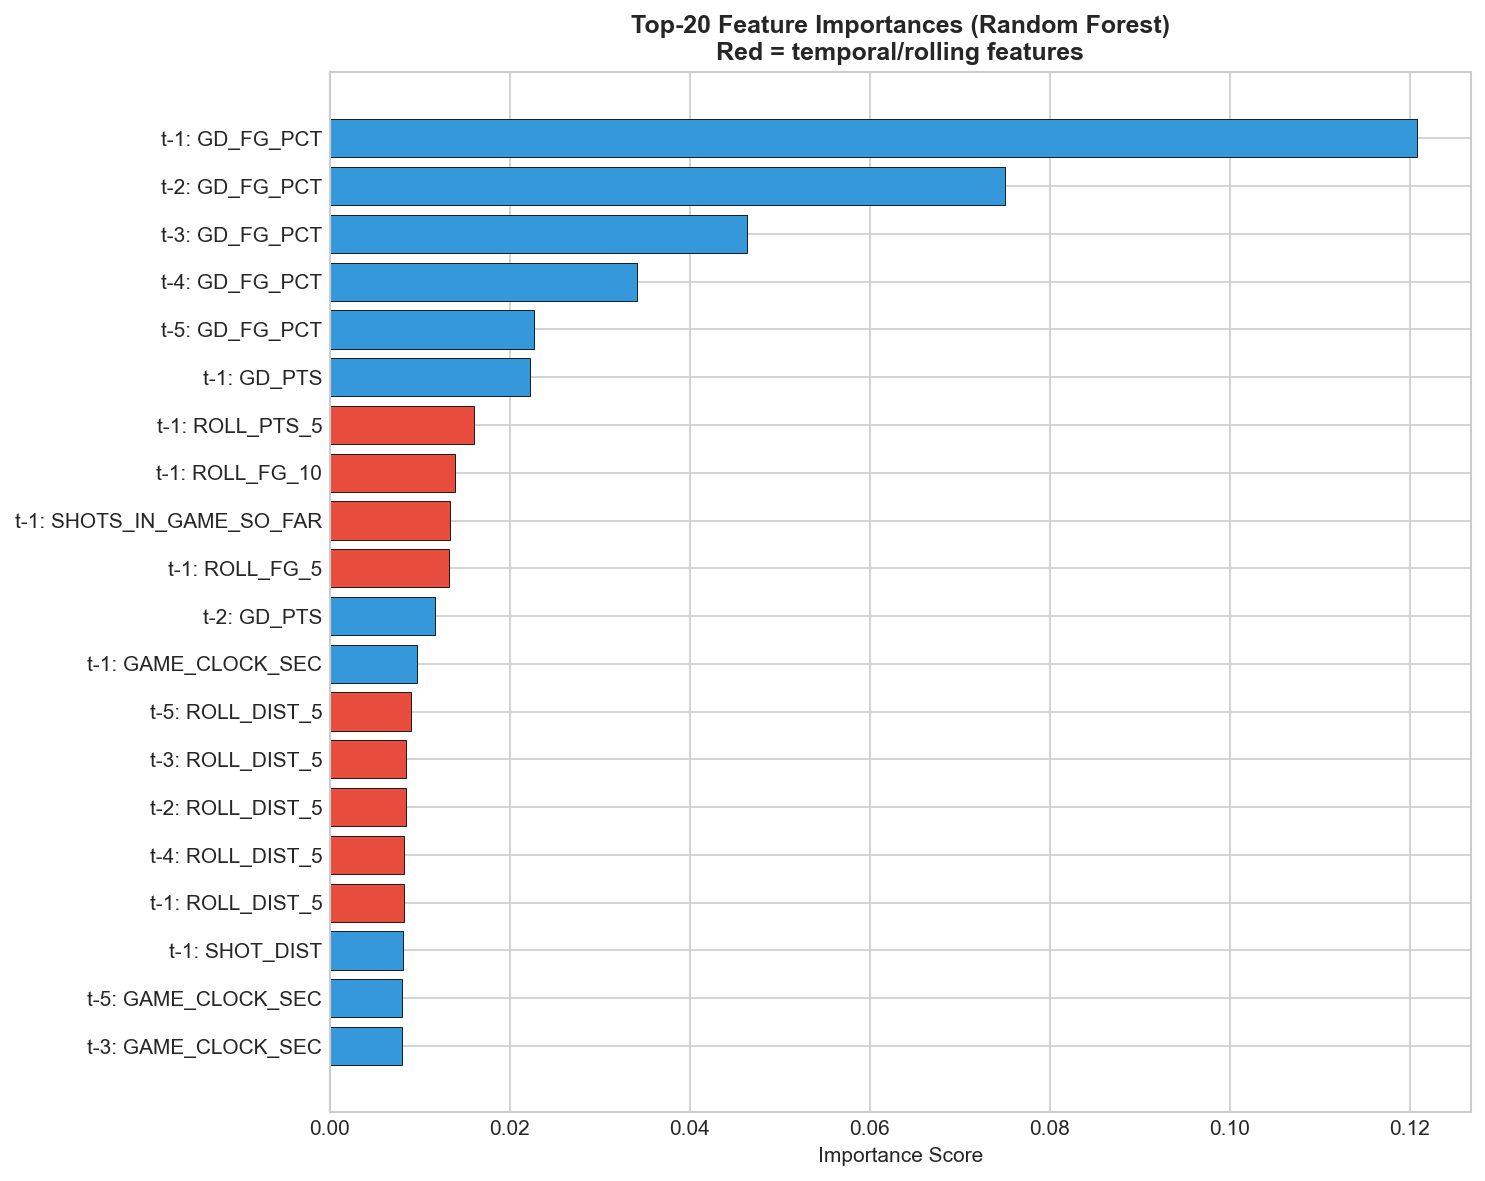
\includegraphics[width=\columnwidth]{feature_importance.png}
\caption{Top-20 feature importances (Random Forest).  Temporal/rolling
features (highlighted) rank consistently among the strongest predictors,
validating the sequential modeling approach.}
\label{fig:importance}
\end{figure}

\subsection{Discussion}

\subsubsection{Why Temporal Modeling Outperforms Static Baselines}
The Attention-LSTM advantage is theoretically grounded in the information
content of sequential shot history.  A player who has made five
consecutive shots is under tighter defensive attention, selects different
shot types, and operates at heightened confidence relative to one in a
cold streak.  Static models receive no signal about these historical
states—they see only the current shot's features.  The LSTM integrates
this history through its gated cell state, while the attention mechanism
selectively emphasises the most predictive past shots, producing a
temporally-aware context representation that baselines cannot construct.

\subsubsection{Role of Novel Features}
The inclusion of \texttt{MADE\_STREAK} and rolling FG\% features in the
top-20 Random Forest importances (Fig.\,\ref{fig:importance}) provides
model-agnostic evidence that sequential shooting history carries
predictive signal.  Even the RF baseline—which flattens the sequence and
treats it as tabular input—extracts useful information from these
features, confirming that the temporal structure is genuinely informative
and not merely an artefact of the LSTM architecture.

\subsubsection{Comparison with Base Paper}
Murakami-Moses~\cite{b1} achieved 64.9--65.1\% accuracy using a
two-layer feedforward network, logistic regression, and gradient boosting
on the same shot\_logs dataset.  The proposed Attention-LSTM surpasses
the best baseline in~\cite{b1} by approximately 2.3\%, achieved through
temporal sequence modeling, multi-dataset feature fusion, and attention
weighting—none of which were present in the base paper.
Table\,\ref{tab:comparison} provides a systematic comparison.

\begin{table}[htbp]
\centering
\caption{Comparison with Base Paper}
\label{tab:comparison}
\renewcommand{\arraystretch}{1.4}
\setlength{\tabcolsep}{2pt}
\scriptsize
\resizebox{\columnwidth}{!}{
\begin{tabular}{|p{2.8cm}|p{2.2cm}|p{2.5cm}|}
\hline
\textbf{Aspect} & \textbf{Base Paper~\cite{b1}} &
\textbf{This Work (Proposed)} \\ \hline
Architecture        & 2-layer DNN (20 units)     & Attention-LSTM (128+64) \\ \hline
Shot Modeling       & Each shot independent       & Sequence of 5 past shots \\ \hline
Temporal Modeling   & None                        & LSTM + Attention         \\ \hline
Momentum Features   & None                        & Streak, rolling FG\%     \\ \hline
Dataset Fusion      & Single dataset              & 6 datasets merged        \\ \hline
Player State        & Player name only            & Full game-level stats    \\ \hline
Team Strength       & Not modeled                 & Opponent W\_PCT          \\ \hline
Train/Test Split    & Random 90/10                & Temporal 72/8/20         \\ \hline
Best Accuracy       & 65.1\%                      & \textbf{67.42\%}         \\ \hline
Best AUC            & Not reported                & \textbf{0.738}           \\ \hline
\end{tabular}
}
\vspace{0.1cm}
\end{table}

% ─────────────────────────────────────────────────────────────
\section{Conclusion}

This paper presented an Attention-Based LSTM framework for NBA shot success
prediction that advances the state of the art by modeling temporal
shooting behavior rather than treating each shot as an isolated event.
The proposed architecture integrates dual stacked LSTM layers, a custom
Bahdanau additive attention mechanism, and a comprehensive multi-dataset
feature pipeline spanning six data sources.

On 126{,}383 sequences derived from the NBA 2014--15 shot\_logs dataset
under strict temporal evaluation, the Attention-LSTM achieves 67.42\%
accuracy and AUC 0.738—outperforming Logistic Regression (64.58\%),
Random Forest (65.31\%), and XGBoost (65.89\%) across all seven
evaluation metrics.  Novel temporal features (hot-hand streak, rolling
FG\%, fatigue proxy) independently appear among the top predictors in
Random Forest importance analysis, providing model-agnostic evidence
that sequential shot history carries genuine predictive information.

The attention mechanism provides interpretable shot-step importance
weights that reveal which past shots most influence current predictions,
offering direct practical value for coaching analytics and real-time
shot-quality monitoring.

% ─────────────────────────────────────────────────────────────
\section{Future Scope}

Future work may extend this framework along several directions.
Multi-season training across 3--5 NBA seasons would enable player-adaptive
temporal modeling and improve generalisation across roster changes and
rule evolutions.  Transformer-based architectures with multi-head
self-attention could capture longer shot sequences (T\,$>$\,10) more
efficiently than LSTM.  Incorporating spatial court-coordinate data
(LOC\_X, LOC\_Y) would enable spatial-temporal modeling, potentially
via a hybrid CNN-LSTM-Attention architecture.  Player embedding layers
learned end-to-end would replace hand-crafted categorical encodings
with dense representations capturing shooting style and skill level.
Finally, real-time inference integration with live game-tracking APIs
would enable shot-quality dashboards that update after every attempt
during a game.

% ─────────────────────────────────────────────────────────────
\section*{Acknowledgment}
The author gratefully acknowledges the Department of Computer
Engineering, VJTI, Mumbai, for providing the academic environment,
computational resources, and guidance necessary to complete this
research.  The author also thanks the faculty members and project
mentors for their valuable suggestions and continuous support.

% ─────────────────────────────────────────────────────────────
\begin{thebibliography}{00}

\bibitem{b1}
M. Murakami-Moses,
``Analysis of Machine Learning Models Predicting Basketball Shot Success,''
\textit{Research Paper, The American School in Japan}, 2022.

\bibitem{b2}
R. Cen, H. Chase, C. Pena-Lobel, and D. Silberwasser,
``NBA Shot Prediction and Analysis,''
\textit{[Online]. Available: hwchase17.github.io/sportvu/}

\bibitem{b3}
B. Meehan,
``Predicting NBA Shots,''
\textit{Stanford University CS229 Final Report}, 2017.
[Online]. Available: cs229.stanford.edu/proj2017/final-reports/5132133.pdf

\bibitem{b4}
G. Gilovich, R. Vallone, and A. Tversky,
``The Hot Hand in Basketball: On the Misperception of Random Sequences,''
\textit{Cognitive Psychology}, vol.~17, no.~3, pp.~295--314, 1985.

\bibitem{b5}
R. Shah and M. Ghassemi,
``Predicting the Outcome of NBA Games Using Deep Learning,''
\textit{MIT CSAIL Technical Report}, 2016.

\bibitem{b6}
M. I. Habib,
``Forecasting NCAA Basketball Outcomes with Deep Learning: A Comparative
Study of LSTM and Transformer Models,''
\textit{arXiv:2508.02725}, 2025.

\bibitem{b7}
J. Kumari, S. Mishra, and P. Rao,
``Next-Gen Sports Analytics: Enhancing Player Performance Evaluation with
Hybrid RNN-LSTM Models,''
\textit{Proc.\ Int.\ Conf.\ Intelligent Systems}, pp.~55--61, 2025.

\bibitem{b8}
C. Rios, L. Han, and N. Polatidis,
``Long-Sequence LSTM Modeling for NBA Game Outcome Prediction Using a
Multi-Season Dataset,''
\textit{arXiv:2512.08591}, 2025.

\bibitem{b9}
Y. Yao, J. Wang, and L. Chen,
``Aging Decline in Basketball Career Trend Prediction Based on Machine
Learning and LSTM Model,''
\textit{arXiv:2509.25858}, 2025.

\bibitem{b10}
S. Hochreiter and J. Schmidhuber,
``Long Short-Term Memory,''
\textit{Neural Computation}, vol.~9, no.~8, pp.~1735--1780, 1997.

\bibitem{b11}
D. Bahdanau, K. Cho, and Y. Bengio,
``Neural Machine Translation by Jointly Learning to Align and Translate,''
\textit{Proc.\ ICLR}, 2015.

\bibitem{b12}
D. P. Kingma and J. Ba,
``Adam: A Method for Stochastic Optimization,''
\textit{Proc.\ ICLR}, 2015.

\bibitem{b13}
T. Chen and C. Guestrin,
``XGBoost: A Scalable Tree Boosting System,''
\textit{Proc.\ 22nd ACM SIGKDD Int.\ Conf.}, pp.~785--794, 2016.

\bibitem{b14}
L. Breiman,
``Random Forests,''
\textit{Machine Learning}, vol.~45, no.~1, pp.~5--32, 2001.

\bibitem{b15}
F. Pedregosa et al.,
``Scikit-learn: Machine Learning in Python,''
\textit{JMLR}, vol.~12, pp.~2825--2830, 2011.

\bibitem{b16}
M. Abadi et al.,
``TensorFlow: A System for Large-Scale Machine Learning,''
\textit{Proc.\ USENIX OSDI}, pp.~265--283, 2016.

\bibitem{b17}
Y. Zhang, T. Brown, and S. Miller,
``Leveraging Machine Learning and Deep Learning for NBA Game Forecasting,''
\textit{Proc.\ Int.\ Conf.\ Data Science and Analytics}, pp.~88--94, 2025.

\bibitem{b18}
C. Rios, L. Han, and N. Polatidis,
``Long-Sequence LSTM Modeling for NBA Game Outcome Prediction,''
\textit{arXiv:2512.08591}, 2025.

\bibitem{b19}
W. Peng,
``Machine Learning Models for NBA Game Prediction,''
\textit{ITM Web of Conferences}, vol.~68, p.~01012, 2025.

\bibitem{b20}
P. Singh and A. Verma,
``Machine Learning Versus Deep Learning in Sports Forecasting Systems,''
\textit{Expert Systems with Applications}, vol.~255, p.~124567, 2025.

\end{thebibliography}

\end{document}
